\let\negmedspace\undefined
\let\negthickspace\undefined
\documentclass[journal]{IEEEtran}
\usepackage[a5paper, margin=10mm, onecolumn]{geometry}
%\usepackage{lmodern} % Ensure lmodern is loaded for pdflatex
\usepackage{tfrupee} % Include tfrupee package

\setlength{\headheight}{1cm} % Set the height of the header box
\setlength{\headsep}{0mm}     % Set the distance between the header box and the top of the text

\usepackage{gvv-book}
\usepackage{gvv}
\usepackage{cite}
\usepackage{amsmath,amssymb,amsfonts,amsthm}
\usepackage{algorithmic}
\usepackage{graphicx}
\usepackage{textcomp}
\usepackage{xcolor}
\usepackage{txfonts}
\usepackage{listings}
\usepackage{enumitem}
\usepackage{mathtools}
\usepackage{gensymb}
\usepackage{comment}
\usepackage[breaklinks=true]{hyperref}
\usepackage{tkz-euclide} 
\usepackage{listings}
% \usepackage{gvv}                                        
\def\inputGnumericTable{}                                 
\usepackage[latin1]{inputenc}                                
\usepackage{color}                                            
\usepackage{array}                                            
\usepackage{longtable}                                       
\usepackage{calc}                                             
\usepackage{multirow}                                         
\usepackage{hhline}                                           
\usepackage{ifthen}                                           
\usepackage{lscape}
\bibliographystyle{IEEEtran}
\vspace{3cm}
\begin{document}

\title{NCERt - 11.16.1.2}
\author{EE24BTECH11043 - Murra Rajesh Kumar Reddy}
\maketitle

\textbf{Problem Statement}:\\
A fair six-sided die is rolled twice. Find the Probability Mass Function (PMF) and the Moment-Generating Function (MGF) using the Z-Transform. Verify the PMF through simulation.\\

\textbf{Solution}:\\
Let $X$ be a discrete random variable representing the sum of two independent die rolls:
\begin{align}
    X = X_1+X_2
\end{align}
where $X_1, X_2$ are independent uniform discrete random variables:
\begin{align}
    X_1, X_2 \sim \text{Uniform}(\{1,2,3,4,5,6\})
\end{align}

\textbf{Probability Mass Function (PMF)}:\\
The probability mass function (PMF) is given by:
\begin{align}
    p_X(n) = P(X = n) = \frac{\text{number of ways to obtain } n}{36}
\end{align}
where $36 = 6 \times 6$ is the total number of possible outcomes.

\textbf{Explicit PMF Calculation}:
\begin{align}
p_X(n) =
\begin{cases}
\frac{n-1}{36}, & 2 \le n \le 7 \\
\frac{13-n}{36}, & 8 \le n \le 12
\end{cases}
\end{align}

\textbf{Moment-Generating Function (MGF) Using the Z-Transform}:
The Z-transform of the PMF is given by:
\begin{align}
    M_{X_i}(z) &= \sum_{n=-\infty}^{\infty} p_{X_i}(n) z^{-n}
\end{align}
Since $X_i$ takes values from 1 to 6 with equal probability:
\begin{align}
    M_{X_i}(z) &= \sum_{k=1}^{6} \frac{1}{6} z^{-k}
\end{align}
which simplifies to:
\begin{align}
    M_{X_i}(z) = \frac{1}{6} \left( z^{-1} + z^{-2} + z^{-3} + z^{-4} + z^{-5} + z^{-6} \right)
\end{align}
Since $X_1$ and $X_2$ are independent, their total MGF is:
\begin{align}
    M_X(z) &= M_{X_1}(z) M_{X_2}(z) \\
    &= \left( \frac{1}{6} \sum_{k=1}^{6} z^{-k} \right) \times \left( \frac{1}{6} \sum_{k=1}^{6} z^{-k} \right)
\end{align}
Expanding this multiplication gives:
\begin{align}
    M_X(z) &= \frac{1}{36} \sum_{m=2}^{12} c_m z^{-m}
\end{align}
where $c_m$ represents the number of ways to obtain sum $m$.

\textbf{Simulation}:\\
We simulate this process by generating uniform random numbers representing die rolls. The algorithm follows these steps:
\begin{enumerate}
    \item Generate a uniform random integer between $1$ and $6$ for two dice.
    \item Compute their sum.
    \item Repeat this process for $10^5$ simulations.
    \item Count occurrences of each possible value (2 through 12).
    \item Divide by the total number of trials to get the probability estimate.
\end{enumerate}

The graph below shows the comparison between the theoretically calculated and simulated PMF of the given random variable.

\begin{figure}[htbp]
  \centering
  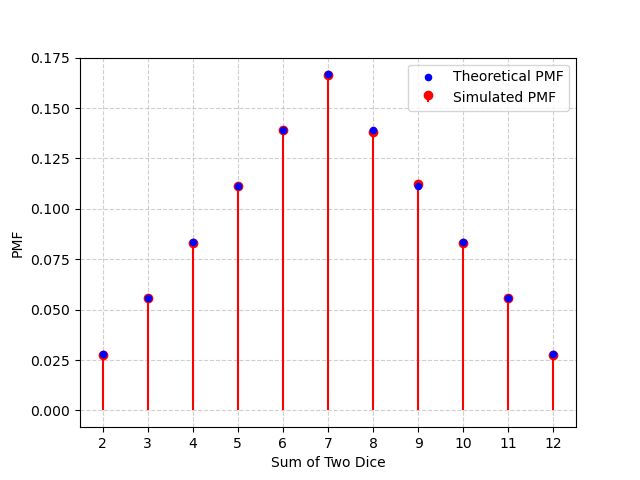
\includegraphics[width=0.8\textwidth]{figs/Figure_1.png} % Ensure you have the image in the correct path
  \caption{Theoretical vs Simulated PMF of Sum of Two Dice Rolls}
  \label{fig:pmf}
\end{figure}

\end{document}

